\documentclass[11pt,  letterpaper]{article}

\usepackage{mathpazo}
\usepackage{fontspec}
\setmainfont{TeX Gyre Pagella}

\input{boilerplate}

\title{\textbf{Asymmetries in Cricket \\ \vspace{5pt} \large{The Effects of Winning the Toss on Winning the Match}}\thanks{This paper incorporates some of the text and 
results from Sood \& Willis's (2019) working paper: ``Fairly Random: The Impact of Winning the Toss on the Probability of Winning.'' The authors thank Matt Blackwell, 
Andrew Gelman, Donald Green, Jens Hainmueller, and Daniel Stone for their comments and suggestions. We are grateful to Sajan Mehotra for outstanding research assistance. 
% The first three authors contributed roughly equally to the research design, data collection, and implementation of the whole project, and are listed alphabetically. Acharya
% contributed to the research design and interpretation of results.
}}

\author{
Apoorva Lal\thanks{Dept.~of Political Science, Stanford University;  \textsf{apoorval@stanford.edu}.} \;\;
Derek Willis\thanks{News applications developer at ProPublica;  \textsf{dwillis@gmail.com}.}  \;\;
Gaurav Sood\thanks{Independent researcher;  \textsf{gsood07@gmail.com}.} \;\;
Avidit Acharya\thanks{Dept.~of Political Science and Graduate School of Business, Stanford University; \textsf{avidit@stanford.edu}.}
}
\date{\today}


%\usepackage[
%  backend=biber,
%  style=authoryear,
%  citestyle=authoryear,
%  ]{biblatex}
%\addbibresource{biblio.bib}
%\renewbibmacro{in:}{}

\begin{document}

\maketitle

\begin{abstract}

In cricket, which team bats first is determined by a toss. Does the team that wins the toss have an advantage over the other team? We find that, on average, the effect of winning the toss on winning the match is essentially nil in international limited-overs daytime matches but substantial (3.3 percentage points) in day/night matches. In Test cricket, the advantage is even larger (4.9 percentage points). The advantage has exploded in the last decade (to nearly 15 percentage points) after a steady decline. Surprisingly, the effect of the toss does not appear to vary between competitive and non-competitive pairings of teams. And as for the decision to bat or field first, we find the win-loss differential is significantly larger for teams that elect to field; the advantage is negligible among those that elect to bat. Lastly, and perhaps most surprisingly, in rain-delayed matches in which the chasing team's total is adjusted by the Duckworth-Lewis formula, we find that teams that elected to bat first did just as well as those that elected to field first.


\smallskip

\textbf{Key words:} cricket, fairness, randomization

%\textbf{JEL codes:} C72
\end{abstract}



% #### ##    ## ######## ########   #######
%  ##  ###   ##    ##    ##     ## ##     ##
%  ##  ####  ##    ##    ##     ## ##     ##
%  ##  ## ## ##    ##    ########  ##     ##
%  ##  ##  ####    ##    ##   ##   ##     ##
%  ##  ##   ###    ##    ##    ##  ##     ##
% #### ##    ##    ##    ##     ##  #######

%
\section{Introduction}
In a competitive sport, every little thing matters. Yet, many sports leave some large levers out of the reach of the teams and in the
hands of fate. In cricket, one such lever---the toss---has been the subject of much attention. In many matches, commentators and cricket enthusiasts claim that there is a definite advantage to either bowling or batting first.\footnote{See, for example, the \href{https://www.quora.com/How-much-does-a-toss-matter-to-a-game-of-cricket}{Quora page on ``How much does a toss matter to a game of cricket?''}} The advantage is also often pointed to by the captains in the pre-toss interview and by the captain of the losing team in the post-match interview. To wrest the advantage, the captain merely needs to pick the side of the coin that will be left facing the sky after the toss and choose whichever one---batting second or batting second---gives the greater advantage.

In this paper, we measure how well teams have been able to capitalize on any advantage conferred by winning the toss. Since the only consequence of the toss is letting the toss-winning side decide whether to bat or field first, we also attempt to measure the advantage of electing to bat first. To answer these questions, we collected data on over 35,000 cricket matches across four formats (First Class, ODIs, T20s, and tests) played over the course of more than one hundred fifty years. (To our knowledge, this is the most comprehensive professional cricket match dataset to date.)

Winning the toss increases the chances of winning the match by 1.8 percentage points: toss winners win 39.2\% of the time and lose 37.4\% of the time, with the remaining share being draws or ties. The effect of winning the toss is the largest in tests, where it is 4.9 percentage points and is smallest in ODIs and T20s, where it is essentially zero. That being said, in ODIs and T20s that are day/night matches, the effect of winning the toss is 3.3 percentage points, whereas, in the day-time matches, the effect is a precise zero.

The effect of toss in the ODIs has remained relatively stable since the 1980's when the one-day format first became popular. In tests, however, the importance of the toss has varied considerably. The effect of winning the toss in test cricket was a little over five percentage points before 1990. It then dropped nearly to 0 from 1990 to 2010. In the last decade, however, it has exploded, averaging 14.5 percentage points. Counter to conventional wisdom, the effect of winning the toss is relatively similar across continents, though the toss appears less important on European and African wickets than elsewhere. The effect on Aussie and Kiwi wickets (3 percentage points) is not substantially different from its effect on South Asian wickets (2.8 percentage points) but is higher than its effect on European and African wickets (1.1 and 0 percentage points respectively).

In sports like soccer, the conventional wisdom is that the toss is inconsequential \citep{csato2020comparison}. In cricket, it is believed that the toss has little significance in lopsided matches that have clear favorites and underdogs. For example, it is thought to be less relevant in an India-Ireland match than in an India-Australia match. For this reason, we look at the effect of the toss separately in subsamples where teams are similarly ranked according to ICC ELO ratings and where their ratings differ by more substantially. We find that the effect of the toss doesn't vary by how well matched the teams are. Since ELO ratings are available only for matches played in recent decades, these findings (along with our finding that influence of the toss has declined over time) suggest that the toss has little influence in modern cricket.

An important caveat about the null findings is in order, however. Our empirical approach cannot tell whether the effects are nil because the toss is unimportant or because the toss is important, but that (modern) teams have not been able to capitalize on the advantage. The toss may matter quite a bit in principle, but we would only be able to observe its effect if a team is able to use the information on the conditions of play and how it pairs strategically against the opposing team to be able to make the optimal decision of whether to bat or field first. If teams simply do not have this knowledge and are often choosing poorly, then we would not see any ``toss effects.'} So, when we refer to ``toss effects'' in this paper, what we are measuring is not whether there is an advantage to winning the toss in principle, but whether any such advantage is exploited in practice.

\footnote{The median rating is 17, so a cutoff of 15 roughly splits the sample of matches in which we have ratings for both teams in two halves.}

%Another way to benchmark the effect of the toss is to compute it in
%terms of ``run- or wicket-advantage.'' To do this, we consider ODI
%and T20 matches, and estimate [.Apoorva: describe the methodology
%that we discussed here]. We find that the effect of winning the toss
%and electing to bat first is an [X] run advantage. In other words,
%the effect of the toss in these instances is nullified only by
%allowing the chasing team to start their innings with [X] runs
%already on the board. Similarly, the effect of winning the toss and
%electing to field first is a [Y] run advantage, so that the effect is
%nullified only if we make the chasing team start with [-Y] runs on
%the board. \todo{We had an idea here that I vaguely recall of how to
%address the complication that if a team loses all ten wickets, then
%we don't observe its 50 over total.}

With this, we turn to the batting first decision. When pitch and weather conditions are hard to read, and it is not obvious that fielding first has a clear advantage, many cricket commentators suggest that batting first is the appropriate choice: get runs on the board, and put the opposing team under psychological pressure by having them chase the target, worrying about ``required run rates,'' etc. We see that the effect of winning the toss on batting first is 13 percentage points. If one team bats, the other team must field, so this translates to saying that among toss winners, 56.5\% of the teams elect to bat, and the remaining 43.5\% choose to field. Thus, compared to the case where teams are randomly assigned to bat, i.e., the case in which the toss has no effect on the batting decision, toss-winning teams bat an excess of 6.5\% of matches. 

However, we find that of the toss winners that elected to bat, only 38.1\% won the match compared to 37.9\% that lost--- a small difference of 0.2 percentage points. On the other hand, of the toss winners that elected to field, 40.8\% won the match compared to 36.9\% that lost--- a larger difference of 3.9 percentage points. This means that 94\% of the 1.8 percentage point effect of winning the toss can be attributed to instances in which the toss winning team elected to field, and only 6\% of the effect can be attributed to the toss winning team electing to bat. This suggests that teams are better able to capitalize on the toss by electing to field when it is advantageous to do so. 
%
%Combining this with the fact that we saw the reduced form effect of the toss on the outcome of the match to be 1.8 percentage points, we can uncover the average effect of batting first on the so-called ``complier'' teams: those that got to bat (because they won the toss) that would not have batted if batting first were randomly assigned \citep{angrist1996identification}. Since winning the toss results in a 0.9\% excess of match wins (from the benchmark case in which the toss has no effect), the effect of batting first in this complier population is 0.9/6.5 = 13.9 percentage points. This is the instrumented effect of winning the toss-- or, the rate at which the excess decisions to bat were converted into excess wins.\footnote{Since the choice to field first is the perfectly colinear inverse of the choice to bat first, flipping the sings of all of our estimates gives the instrumented effect of electing to field first. For example, the instrumented effect of electing to field first is -13.9 percentage points.} 
%
%This conversion rate is different in sign and considerably larger than the naive difference in win
%probabilities between teams that bat first and those that don't, which is $-1.6$ percentage points. Since the rules of cricket imply that the toss cannot affect the outcome of the match other than through the decision of the toss-winning team to bat or field, this discrepancy is likely due to the complier population being very different from the never-taker or always-taker populations that form the bulk of our team-match data. The IV estimates are thus
%telling us that some teams in some matches are able to take advantage of the decision to bat first when the batting choice really matters.

We also look at how the toss advantage breaks down between teams that elected to bat versus those that elected to field within the various subgroups mentioned above and others. Perhaps the most striking result from this analysis for many cricket followers is that there does not appear to be the case that toss winners that elect to bat first do better than those that elected to field first in rain delayed matches where the chasing total is adjusted according to the \citet{duckworth1998} formula. 

Our results are pertinent to debates on how cricket should be governed. One argument is that since the toss is random, no team is advantaged by the format prior to the toss; and in fact the luck of the toss along with the strategic choice to bat first or second are integral parts of the game--- not very different from the luck of weather affecting the teams differently. 
%or the strategic choices that captains make as to how to set the field, or the order in which they deploy their batsmen.
An alternative argument, however, is that the toss is problematic because it advantages one team over the other even before the first ball is bowled; and care should be taken to mitigate this asymmetry--- for example, by making cricket pitches more durable so that they don't deteriorate so much so that batting on the final day of a test match is miserable. Otherwise, the toss-winning team could exploit this advantage by batting first, reducing the chance that it has to endure this misery. Moreover, the fact that no side is advantaged \emph{ex-ante} if the toss is random is not enough to justify not correcting any asymmetry created by the toss. In fact, the rules of cricket already try to correct the asymmetry between teams that bat first and those that bat second in one particular instance: In rain-delayed one-day matches, the Duckworth-Lewis formula is used to set a new target for the chasing team.\footnote{The argument that no side was advantaged \emph{ex-ante} could have been used to justify not doing any correction in such rain-delayed matches, and simply declaring that the team that batted first won the match because the chasing team was unable to reach its target. But the designers of one-day cricket were clearly unwilling to allow the bad luck of weather to have this much influence on the game. If addressing the misfortunes of weather are important, it may also be important to address the misfortune of losing the toss.} 

For those who take this latter viewpoint, a straightforward policy prescription that comes out of our analysis is that, at least for ODIs, day-night matches should be avoided. In general, when new formats are introduced (such as the recent introduction of T20s) care should be taken to ensure the toss has little effect. The designers of cricket should always consider ways of leveling the playing field for the competing teams starting from the point at which the game really begins--- the moment the first ball is bowled. 

We do not address these optimal design questions in this paper, but our results are relevant to these issues depending on what the designers of cricket seek to optimize. %However, at the end of the paper, we propose (and discuss the possible consequences of) a subtle change to the rules governing the toss: Rather than tossing a coin to confer the choice to bat first or second upon the captain of the toss-winning team, umpires may consider simply tossing a coin to determine which team must bat first.


% ########     ###    ########    ###
% ##     ##   ## ##      ##      ## ##
% ##     ##  ##   ##     ##     ##   ##
% ##     ## ##     ##    ##    ##     ##
% ##     ## #########    ##    #########
% ##     ## ##     ##    ##    ##     ##
% ########  ##     ##    ##    ##     ##


\section{Data}

\subsection{Creating the sample}

We obtained data on cricket matches from the ESPN Cricinfo website, which provides coverage of international and many domestic matches,
and maintains statistics on a wide variety of matches across formats.\footnote{Information on all available matches was downloaded in June 2020 using a purpose-built parsing library available at \href{https://github.com/dwillis/python-espncricinfo}{https://github.com/dwillis/python-espncricinfo}. The data will be available as a separate repository available at \href{https://github.com/dwillis/cricket-stats}{https://github.com/dwillis/cricket-stats}.} 

We focus on four types of formats: T20, ODI, Test, and First Class matches for both men's and women's teams.\footnote{We do not include the List A matches that are not ODIs or T20s, which are often considered a less professional category (with worse data recording) than the formats that we include.} The data are a near census of the relevant population, excluding only scheduled matches that were abandoned without the toss being conducted, and a small number of limited-overs matches in which the minimum number of overs that must be bowled to establish a result was not met.\footnote{In ODIs, for example, each side must bat at least 20 overs for a result to be declared. We have no reason to suspect that the small matches that were excluded because they did not meet this threshold could be biased enough to affect our conclusions. We drop 426 matches recorded as ``no result,'' 3 matches that are recorded as ``abandoned'' or ``canceled,'' and another three that don't record who bat first. The former constitutes the largest exclusion we make and appears to be comprised of matches canceled for idiosyncratic reasons, ranging from the \href{https://www.espncricinfo.com/series/shell-tri-series-1991-92-61203/australia-women-vs-england-women-final-66975/full-scorecard}{a team being unable to bat because of the weather} to cancellations because of \href{https://www.espncricinfo.com/series/australia-tour-of-pakistan-1982-83-61392/pakistan-vs-australia-3rd-odi-64196/full-scorecard}{unwanted audience participation}. This results in us dropping approximately 0.07\% of matches.}

Our final sample comprises of 35,357 cricket matches across four formats played over the last 150 years. We report the distribution of matches over time and by type in Figure \ref{fig:timeseries_decomp}. As the figure shows, the number of matches has exploded over the last two decades, largely due to the introduction of the enormously popular Twenty-20 (T20) format of the game both in both international and domestic tournaments. T20 matches constitute over a quarter of all matches played in the last decade.

% subsubsection data_collection (end)

\subsection{Is the toss random?}

Since our analysis will be based on the assumption that the coin toss is random, we start by examining this assumption.\footnote{Prior work in the sports analytics of cricket by \citet{shafqat2015analysis} and \citet{dawson2009bat} conditions on post-treatment variables, whereas we use only the randomization of the toss to identify toss effects.} Is there any evidence that the coin toss is somehow rigged--- for example, with the home side enjoying the rub of the green more often? In order to study this, we compare the rates at which home teams, teams that won the toss in their last match, and underdogs (defined as the lower-ranked team whenever rankings are available for both teams) win the toss relative to their opponents. 

To examine whether the toss is rigged, we compute the odds of seeing as many successes in the same number of draws of a sequence of independent Bernoulli random variables with parameter 0.5. For example, home teams have won 50.81\% of tosses in the 6377 matches for which we have data. The likelihood of tossing a fair coin 6377 times and getting at least this percentage of heads is 20.1\%. This chances appears low, but not eyebrow-raisingly so. We find that toss wins are even more balanced for teams that won and lost the last toss, and for teams that are underdogs and favorites. Table \ref{table: balance} reports these balance results. 

That said, we do see one potential source of concern. We find that teams that share their nationality with at least two of the three umpires of the match win 51.3\% tosses in the 4044 international matches for which we have this data. The likelihood that tossing a fair coin 4044 times and and getting at least this share of heads is only 10\%. This number is certainly low enough to raise some eyebrows. That said, the practice of allowing home-team umpires in international matches ended in 1992, and so these issues are less relevant in recent decades which comprise the bulk of our sample. 

In addition, a rigged toss in favor of the home team would bias estimates of the advantage of winning the coin toss to the extent that it is
correlated with ability. If stronger teams win more tosses, estimates of the advantage of the coin toss would be inflated upwards. And vice versa, if otherwise. We do not have good reasons to think that there is a correlation. So for now, we proceed as if the toss is random.


% robust standard errors and report these estimates in
% table~\ref{table:baltab} alongside the number of matches used to test
% for balance. Wefail to reject the null that the toss is random.



%N = 6377
%Wins = 3240 home team wins
% prob succes = 50.81
% p value = 20.14\%.

%Wins = 17189
%N = 34283
%50.14
%p value = 0.6114

%Underdog = lower ranked team in any dyad with nonmissing ranking info (so int'l matches)
%Underdog won = 2001
%N = 4054
%Win prob = 49.36\%
%p value = 0.4231





% % latex table generated in R 3.6.3 by xtable 1.8-4 package
% Wed Dec  2 21:53:13 2020
\begin{table}[ht]
\centering
\begin{tabular}{lrrrrr}
  \hline
 & Increased odds of winning toss & SE & T-stat & p-value & N \\ 
  \hline
Home Team & 0.02 & 0.01 & 1.82 & 0.07 & 6377.00 \\ 
  Won last toss & 0.00 & 0.00 & 0.83 & 0.41 & 34600.00 \\ 
  Underdog & -0.01 & 0.01 & -1.19 & 0.23 & 3975.00 \\ 
   \hline
\end{tabular}
\caption{balance table} 
\label{table:baltab}
\end{table}



% ########  #######   ######   ######
%    ##    ##     ## ##    ## ##    ##
%    ##    ##     ## ##       ##
%    ##    ##     ##  ######   ######
%    ##    ##     ##       ##       ##
%    ##    ##     ## ##    ## ##    ##
%    ##     #######   ######   ######


\section{Do teams exploit the advantage of winning the toss?}

To estimate the advantage of winning the toss, we run regressions on a team $\times$ match level dataset. Let $i$ index teams, and $j$ index matches. $Y_{ij}$ is a dummy for team $i$ winning match $j$, and takes a value of $0.5$ for draws. $Z_{ij}$ is a dummy for team $i$ winning the toss in match $j$. For the main specifications of interest, we estimate regression equations of the form
\begin{equation}\label{eqn:reduced_form}
Y_{ij} = \alpha_0 + \tau Z_{ij} + \gamma_i + \delta_t +
\psi_k + \varepsilon_{ij}
\end{equation}
which includes fixed effects for teams $\gamma_i$, time $\delta_t$, and match-type $\psi_k$, so that all variables can be interpreted as residuals from partialing out team, match-type, and time fixed effects. Since unobservable factors are correlated across opposing teams in the same match, we cluster the standard errors at the match level.

We report results in Table \ref{table:reduced_form}. We progressively introduce team, match-type, and time period fixed-effects in columns 2, 3, and 4 to make more fine-grained comparisons, and find that results are remarkably stable across specifications. The first column, for example gives
the baseline estimate of the toss effect being 1.8 percentage points in all matches. As we mentioned in the introduction, this effect represents toss winners winning 39.2\% of the time and losing 37.4\% of the time, with the remaining matches being draws. The estimated effect remains at 1.7 percentage points when we progressively add the fixed effects.

We then proceed to examine the effect of the toss withing various subgroups. We report the estimates graphically in Figures \ref{fig:rf_het_TE} - \ref{fig:omni_het_test} with point estimates and sample sizes as annotations. The results are summarized as follows.

\textbf{Format.} Toss effects are most pronounced in test matches followed by first class matches, and are statistically indistinguishable from zero in ODIs and T20s. We estimate the effect of the toss on winning a test match to be 4.7 percentage points, allowing for the fact that many tests end in draws. Given that only 65\% of test matches end with one team winning, the effect of the toss conditional on the match producing a winner is higher: 7.2 percentage points. The effect of the toss in first class matches is 2.3 percentage points. These results support the conventional wisdom among lay cricket followers that the toss grants the greatest advantage in multi-day affairs. Pitches invariably deteriorate over the course of these matches, and the fourth innings in test match is often the most challenging time to bat. The pitch deteriorates far less over the course of a day, or in the case of T20s, a few hours. Our null results for limited over matches also extend \citet{de1998winning}, who, based on analysis of data from 427 international one-day matches conclude that ``winning the toss at the outset of a match provides no competitive advantage.''

\textbf{International vs.~Domestic matches.} Toss effects are virtually the same for international and domestic matches (point estimates are 1.7 percentage points in the former, and 1.9 percentage points in the latter). This is a bit surprising given differential use of cricket formats differs in international and domestic matches (for example, there are no domestic tests), and our findings of heterogeneous effects across formats. 

\textbf{Effects over time.} Toss effects overall appear to have declined over time from a high of 9.9 percentage points in the second half of the 19th century, to 1.4 percentage points in the last decade. We also look at these trends within format. T20s have not been played long enough for us to draw any conclusions about how toss effects have changed over time. But within the other formats, we find that toss effects follow a similar pattern, except that in test cricket there is a peculiar uptick in in the last decade: the toss effect jumps from 0 in the decade before to 14.5 percentage points now.  We investigate potential sources of this variation below  but there are some factors that could be important drivers for which we do not have data. For example, cricketers may have become more fit, and able to play for longer periods without tiring as much as they once did. Pitches now may be more resilient to wear than they once were. Teams may have acquired better knowledge on how to play more effectively whether they bat first or second. Etc.

\textbf{Relative strength.} Common sense suggests that the toss should be less important in lopsided matches where there is one dominant team that is expected to win, whether it bats first or second. It should be more important in competitive matches where the opposing teams are more even in cricketing strength. We define competitive matches as those in which the gap in ELO ratings of the two teams is less than 15 points. Since the median ELO rating difference is 17 points, this threshold roughly splits our sample of matches for which we have ELO ratings for both teams in two halves. Surprisingly, we find the toss effect to be nearly the same, and indistinguishable from zero within both competitive and noncompetitive matches even when we look at tests and international ODIs separately (these are the two formats for which ELO ratings apply). Part of the reason for this is that the ELO ratings are available only for recent years, and we saw above that toss effects have declined over time. We also perform an omnibus test of treatment effect heterogeneity by estimating sorted partial effects \citep{chernozhukov2018sorted,chen2019sortedeffects} with respect to ranking and result history, and find minimal evidence for effect heterogeneity. 

\textbf{Continents.} We find that toss effects vary only somewhat across continents, hovering around 2.5 percentage points for matches played in Asia, Oceania, and the Americas (though the estimates for the Americas are noisier in part due to the smaller number of matches played there). In Europe (mainly England) the toss effect is only 1.1 percentage points (though we do not rule out a null effect), and in Africa it is essentially zero. Overall, despite there being much talk about the different nature of wickets across the world, with wickets in certain regions being drier, or stickier, or subject to more wear, these differences do not seem to translate into substantial toss effect differences at least when we look coarsely at averages.

\textbf{Day/Night matches.} It is often claimed that the toss is more crucial in day-and-night matches. We find some evidence for this. In the limited overs formats where day/night matches take place (ODIs and T20s), the advantage of winning the toss in a day/night match is 3.3 percentage points, whereas the
advantage of winning the toss in a limited overs match played during the day is zero. 

\textbf{Seasonality.} Weather is also thought to have a large impact on the playing conditions in cricket. Cool
overcast weather, for example, is thought to aid swing bowling, especially in English pitches. More generally,
the advantage of winning the toss likely varies by the weather. Although do not have data on
the weather, we can proxy it with seasons. In particular, students of the game suspect that
the advantage of winning the toss in the early English season is especially significant.
There is some evidence of a seasonal pattern for matches played in England, with the advantage of winning the toss
growing over the summer, though the trend is weak and broken in the month of July.

\textbf{Rain delays.} Finally, we look at the differential effects of winning the toss in ODI matches that were rain-delayed, causing the number of overs bowled in the second innings to be adjusted down. We examine the subset of matches where rain-delays result in revised targets computed using the \citet{duckworth1998} method. This method has been the subject of much controversy, with many cricket fans suggesting that it is rigged against the chasing team. To our surprise, we find no evidence that toss winners are able to exploit the possibility of second inning rain delays to their advantage. If anything, we see that the toss-winner has a \emph{disadvantage} of 2.4 percentage points in matches subject to the Duckworth-Lewis adjustment, though this point estimate is statistically indistinguishable from zero \footnote{Toss-winners won 160 out of 333 ODIs with DL adjustment and 3085 out of 6187 ODIs without DL adjustment}. This, however, does not mean that the Duckworth-Lewis method is not rigged against the chasing team; that issue will be discussed further in the next section.



% \begin{table}
% \centering
% \caption{Reduced Form Effect of Toss on win probability by match type}
% 
\begin{tabular}{@{\extracolsep{5pt}}lcccc} 
\\[-1.8ex]\hline \\[-1.8ex] 
 & Domestic & International & Day & Day/night \\ 
\\[-1.8ex] & (1) & (2) & (3) & (4)\\ 
\hline \\[-1.8ex] 
 Win Toss & 0.019$^{***}$ & 0.017$^{*}$ & $-$0.002 & 0.033$^{**}$ \\ 
  & (0.005) & (0.009) & (0.009) & (0.017) \\ 
  Constant & 0.491$^{***}$ & 0.491$^{***}$ & 0.501$^{***}$ & 0.484$^{***}$ \\ 
  & (0.003) & (0.004) & (0.005) & (0.008) \\ 
 \hline &  &  &  &  \\ 
Number of Matches & 24131 & 11226 & 11223 & 3556 \\ 
\hline \\[-1.8ex] 
\end{tabular} 

% \label{table:reduced_form_het}
% \end{table}



% subsubsection heterogeneous_treatment_effects (end)

% \newpage


% ########     ###    ########
% ##     ##   ## ##      ##
% ##     ##  ##   ##     ##
% ########  ##     ##    ##
% ##     ## #########    ##
% ##     ## ##     ##    ##
% ########  ##     ##    ##


\section{Batting versus Fielding First}

\subsection{The Choice to Bat}

The first column of Table \ref{table:iv_table} shows that 49.2\% of teams that batted first won the match, while 50.8\% of teams that fielded first won. The second column shows that among teams that won the toss and batted first, the ``win-loss differential'' is small: these teams won only 0.2 percentage points more frequently than they lost, winning 38.1\% of matches and losing 37.9\% of matches, as reported in the introduction. This win-loss differential is smaller than it is for teams that won the toss and elected to field. The third column of the table shows that these teams won 3.9 percentage points more frequently than they lost: they won 40.8\% of their matches and lost 36.9\% of them. Combining this information with the fact that 56.5\% of teams that won the toss elected to bat (and only 43.5\% elected to field, as implied by the fourth column of the table) this means that 94\% ($= .435 \times .039/.018$) of the 1.8 percentage point advantage to winning the toss that we reported in the previous section can be attributed to the success of toss-winning teams that elected to field. 

These findings are not surprising given the conventional wisdom that captains who are not sure whether they should bat or field first often choose to bat. If a team wins the toss and elects to field, they often have a good reason to do so. It is interesting to ask what these reasons could be. Although we cannot answer this question fully, comparing  the win-loss differentials within subgroups may offer some clues. 

\textbf{Format.} In test matches 72.8\% of teams that win the toss elect to bat, whereas in T20s and ODIs this share is only about 52.9\%. In first class matches it is 56.9\%. It appears that teams err heavily on the side of batting first in longer match formats. 

\textbf{International vs. Domestic matches.} We see no big differences in propensity to elect to bat first across international versus domestic matches.

\textbf{Effects over time.} Historically, toss-winning teams tilted heavily in favor of batting first, but this declines over the course of the 20th century, and now they show no preference (on average) to  bat first. Even for test matches, toss winning teams tend to be tilting less toward batting first than they once did. Pre-1950, more than 90\% of teams that won the toss elected to bat, whereas in the last two decades that number is closer to two-thirds. Perhaps players have gotten more fit and are willing to trade-off expecting to have to bat on the final days of the match in favor of taking advantage of playing conditions that are favorable to fielding first. As for ODIs, captains curiously erred heavily on the side of fielding first in the early decades of the format, but in the last thirty years, they have tilted more towards batting first, with just over half of toss-winning teams electing to bat. 

\textbf{Relative strength.} We see no notable differences in the toss-winning captain's choice to bat first across matches that are lopsided and those in which the teams are more evenly matched. This is especially true in tests, but also appears to be true in ODIs, though a slightly larger share of toss-winning teams elect to bat in matches that are lopsided (54.6\%) in comparison to ones that are less lopsided (51.9\%).

\textbf{Continents.} Toss-winning captains show a preference to bat first in matches played in Oceania and Europe, more so than in other pitches. For example, in Europe (mainly England) $64.9\%$ of toss winning teams elect to bat, and in Oceania this number is $59.9\%$. By contrast, on Asian wickets it is only $50.1\%$. 

\textbf{Day/Night matches.} The ball being harder to see at night afflicts both the night-time batting team, as well as the fielding team, making it prone to dropping catches. But the difficulty for batsmen is probably greater than it is for fielders. Indeed, within the shorter formats, the variation between day matches and day/night matches is greatest when it comes to the choice to bat first. In day/night matches, $59\%$ of toss-winning teams elect to bat first, whereas in day matches just about only half of them do. 

\textbf{Seasonality.} The preference to bat first in England follows a broadly similar trend to the toss effect over the course of the year-- rising steadily over the summer, and drops in September. At its peak in August, top-winning captains choose to bat first $71.9\%$ of the time. At its lowest in April, they choose to bat $57.4\%$ of the time.

\textbf{Rain delays.} Remarkably, there is an overall preference to field first in matches that ended up using the Duckworth-Lewis adjustment: only $43.5\%$ of toss winning teams elected to bat in these matches. If captains are at all able to predict rain (and other) delays, they seem to show a preference to bat a fewer number of overs and chase the adjusted target. 

\subsection{The Difficulty in Estimating the Advantage to Electing to Bat/Field First}

Despite having reported the `reduced form' and `first stage' effects of the toss, we cannot not interpret the ratio of these effects as the causal effect of batting first. If we used the toss as an instrument for batting first, say, we could at best hope to estimate the local average treatment effect (LATE) of electing to bat on winning the match \citep{angrist1996identification}. This is because in our setting  treatment effects likely vary across groups: some teams in some circumstances will be better able to capitalize on the ability to bat or field first.  

However, even the conditions under which the LATE is known to be identified are probably not satisfied in our setting. To see why, first note that our setting has two-sided noncompliance: there are teams that win the toss that bat first, and those that lose the toss that bat first as well. Then, recall that under two-sided noncompliance, the LATE is identified under a monotonicity assumption that rules out defiers. However, defiers are likely to be present in our setting: they correspond to dyads of opposing teams that walk on to the pitch, both intending to field first if they win the toss. In such a setting, the team that wins the toss will chose to field first and the team loses the toss will be compelled to bat first. If these defiers are present, which they likely are, the monotonicity assumption does not hold, and so we cannot assert that the IV estimates are giving us the LATE.

We make these points a bit more concrete. Recall that we saw that 56.5\% of teams that won the toss elect to bat, which corresponds to an excess of 6.5 percentage points over the benchmark case in which the toss has no effect on the batting/fielding decision. In addition, the reduced form estimated effect of winning the toss on winning the match was 1.8 percentage points, implying that toss winners win an excess of 0.9 percent of matches over parity. The instrumented effect of batting first would then be estimated as 0.9/6.5 = 13.9 percentage points.\footnote{Since the choice to field first is the perfectly colinear inverse of the choice to bat first, flipping the sing of this number gives the estimated instrumented effect of electing to field first.}  Can we interpret this as the average rate at which the complier teams that won the toss and elected to bat generated the excess wins? Not really, because these excess wins could have been generated by the defiers making good decisions to field. Since we saw that teams that win the toss and elect to field first have a higher win-loss differential than those that elect to bat first, it would be irresponsible to rule out this possibility. Consequently, it is unlikely the LATE can be identified in our setting.

% \section{Changing the Rules of the Toss}

% We end with a small but potentially important policy proposal that cricket boards might consider. The proposal is to eliminate the choice that the toss confers upon the toss-winning captain. How can this be done? The umpire assigns either of the two opposing captains to take heads, and flips the coin. If the coin lands heads, that captain must bat; otherwise, that captain must field. The captains do not get to make any choices.

% What does this take away from cricket? What problem does it fix? \todo{Guys, we should have a discussion about this!} 

%
%This conversion rate is different in sign and considerably larger than the naive difference in win
%probabilities between teams that bat first and those that don't, which is $-1.6$ percentage points. Since the rules of cricket imply that the toss cannot affect the outcome of the match other than through the decision of the toss-winning team to bat or field, this discrepancy is likely due to the complier population being very different from the never-taker or always-taker populations that form the bulk of our team-match data. The IV estimates are thus
%telling us that some teams in some matches are able to take advantage of the decision to bat first when the batting choice really matters.
%
%Batting first is a strategic decision made by the captain of the team
%that won the toss in any given game. As such, a naive comparison of
%win rates between teams that chose to bat first versus those who
%didn't is unlikely to uncover the causal effect of batting first since
%the treatment (batting) is endogenous. To get around this problem,
%we use the randomly assigned ability to chose to bat first
%afforded to one of the two captains by virtue of winning the toss as
%an instrument for batting first. Note that because the decision to field first is the prefectly colinear inverse of the decision to bat, we can flip the sign of our point estimates to interpret them as the instrumented effects of choosing to field. 
%
%Since after winning the toss, a captain has the choice to bat field, instrumenting for batting first by the coin toss amounts to
%analysing an encouragement experiment with one-sided non-compliance
%. In this context, this corresponds to the outcome
%where the captain that won the toss still chooses to field first. The
%toss readily constitutes a valid instrument--- it
%gives the captain the choice to bat first, and almost certainly
%satisfies the exclusion restriction, as the toss is unlikely to have an independent effect
%on the outcome of the match besides its effect on the order that teams bat.\footnote{The only other possibility is that winning or losing the toss may have a dire psychological effect that directly affects their performance. We believe this to be unlikely.}
%Since we are in the ``just-identified'' case with a single endogenous
%regressor (the choice to bat first) and a single instrument
%(winning the toss), we can recover the causal instrumented effect of batting first as the ratio of the
%reduced-form effect of the toss on win probability divided by the first stage effect of the
%toss on the choice to bat.
%
%These assumptions are sufficient if we assume that the instrumented effect is constant in
%the population. However, we believe this to be an implausible assumption and
%therefore operate in the heterogeneous-effects framework proposed by
%\citet{angrist1996identification}. This necessitates an additional
%assumption--- that of {monotonicity}, which requires that the toss
%only moves batting choices in one direction: teams that would have
%otherwise chosen to bat first don't switch to fielding first upon
%winning the toss.\footnote{Formally, if $D_1$
%is the binary choice to bat upon winning the toss, while $D_0$ is the
%assignment when losing the toss, then monotonicity  assumption is stated as
%$\Prob{D_1 \geq D_0} = 1$.} Despite being unverifiable, this assumption is
%is likely to be valid. By using the instrumental variables (IV) estimator, we are therefore
%estimating the Local Average Treatment Effect (LATE) for
%{compliers} -- teams that are able to harness the
%available information about whether or not it is advantageous to bat
%first, and chooses to do so when it is in fact there is such an
%advantage.\footnote{An alternative formulation of the IV framework
%proposed by
%\citet{heckman2005structural} permits a
%characterisation of treatment selection based on a latent variable
%$U_i$, which yields a monotonicity assumption of the form $D =
%\Indic{U_i \leq p(\vee{X}_i, Z_i)}$, where $U_i$ is an unobserved
%propensity to take treatment (in our setting, choose to bat first
%given available information), and $p(\vee{X}_i, Z_i)$ is the propensity score.
%$U_i$ is normalised to be distributed on the unit interval and encodes
%information about an individual $i$'s treatment choices
%$\SetB{D_i(z)}_{z \in \Sett{Z}}$. This framework allows for
%extrapolation of the LATE into other target parameters.}
%
%We report the naive OLS estimate of the estimated difference in win
%rates in column 1 of Table \ref{table:iv_table}, which is
%counter-intuitively small and negative. In column 2 we estimate this
%specification separately across matches in which the toss-winner
%chooses to bat first, and in column 3 we estimate it in matches in which the toss-winner
%chooses to field first. We find that matches in which the
%toss-winner chooses to field first exhibit a substantial first-batter
%disadvantage, which suggests that captains are doing better than
%choosing randomly between batting and fielding first. We report the
%first stage effect of winning the toss on the choice to bat first in
%column 4, and find that winning the toss increases the probability
%of batting first by 13 percentage points, which is a sizeable effect.
%Columns 5-7 report the IV estimates. We find that in
%contrast to the naive OLS specification, the IV estimate gives a
%sizeable first-batter advantage of between 13.4 and 13.9 percentage
%points across specifications with team- and match-type fixed effects.
%
%Like with the toss, we then proceed to analyse heterogeneity in the instrumented effect. The results are depicted in Figures
%\ref{fig:iv_het_TE1} - \ref{fig:iv_het_TE3}.  
%



%
%
%\subsection{Characterising Compliers} % (fold)
%\label{sub:characterising_compliers}
%
%A complier in our setting is a team that is able to harness the
%available information about whether or not it is advantageous to bat
%first, and chooses to do so when it is in fact there is such an
%advantage. Since the monotonicity assumption rules out defiers,
%we can decompose the sample into {always takers}, {never
%takers}, and {compliers}
%\citep{angrist1996identification,Abadie2003-hj}. The fractions of each of these are given by 
%\begin{align*}
%\pi_{\text{compliers}} & = \Prob{D_1 > D_0 }= \Exp{D | Z = 1} - \Exp{D | Z = 0} \\
%\pi_{\text{always-takers}} & = \Prob{D_1 = D_0 = 1 } = \Exp{D | Z = 0}  \\
%\pi_{\text{never-takers}} & = \Prob{D_1 = D_0 = 0 } = 1 - \Exp{D | Z = 1}
%\end{align*}
%where $D_1$ is a dummy for batting upon winning the toss, $D_0$ is a dummy for batting first upon losing the toss, and $Z \in \{0,1\}$ is the outcome of the toss, with 1 coded as a win.  Applying the above formulae to our sample yields 13\% compliers,
%43.5\% always takers and 43.5\% never takers respectively. This is a small fraction of compilers, suggesting that teams are generally not very adept at capitalizing on the toss. However, it could also be that since a complier is a team-match, match conditions in which the toss would matter may not be that prevalent. We cannot tell. 
%
%To better understand the population of compliers, we apply \citeauthor{Abadie2003-hj}'s (2003) kappa to compute the mean of covariates for compliers. The kappa can be applied to any
%characteristic or outcome to get its mean for compliers by removing
%the means for never and always takers using the kappa weights. %\footnote{Abadie's formulation is
%%considerably more general and applies to any measurable function $g(Y,
%%D, \vee{X})$ with finite variance.
%%$$
%%\Exp{g(Y, D, \vee{X}) | D_1 > D_0} = \frac{\Exp{\kappa \cdot g(Y, D,
%%\vee{X})}}{\Prob{D_1 > D_0}} = \frac{\Exp{\kappa \cdot g(Y, D,
%%\vee{X})}}{\Exp{\kappa}}
%%$$. In our application, $g()$ simply returns $x_i$.
%% }. 
%
%Kappa weights are defined by
%$$
%\kappa = 1 - \frac{D(1-Z)}{1 - \Prob{Z = 1| X}} - \frac{(1-D)
%Z}{\Prob{Z=1|X}}
%$$ where $X$ is a characteristic. We average a characteristic $X$ using kappa weights computed using the
%above expression where $\Prob{Z = 1 | X}$  is estimated using a
%logistic regression \cite[p
%181-183]{angristMostlyHarmlessEconometrics2008}. Applying this procedure to some team-specific
%characteristics yields the averages reported in Tables 4 and 5. We find
%that compliers are marginally more likely to be underdogs (defined as
%the lower rated team in the match, according to ELO ratings), away teams, and teams playing in
%Asia. Among the teams that made the right decision to bat first after winning the toss, 78\% of them were playing day/night matches-- a remarkably high number. This suggests that it is relatively easier to make a good choice of whether to bat or field first in day/night matches. 
%
%Another result that is noteworthy, is that over a quarter of team-match compliers are Australian teams-- by far the highest frequency of any international team. England, Pakistan, South Africa, and India are all essentially tied for second place with a frequency of around 15\% each. What is surprising is how poorly West Indian, Sri Lankan and Kiwi teams do in choosing to bat when it matters. These are strong teams with quite a bit of cricketing experience in comparison to teams like Bangladesh, Kenya and Zimbabwe. And yet they do not seem to enter the complier population at higher rates.\footnote{For this interpretation, the match conditions are unlikely to be driving these differences. What we mean by this is the following. Suppose that Aussie teams are better at capitalizing on choosing to bat or field because Aussie wickets are particularly more likely to provide the playing conditions in which choosing to bat or field matters; and Aussie teams play on Aussie wickets more often than other teams. However, we see that matches played in Asian wickets constitute more than half of the complier population.} 
%
%%estimating the following
%%system of equations in order to uncover the batting advantage:
%%\begin{align}
%%Y_{ij} & = \alpha_0 + \beta D_{ij} + \varepsilon_{ij} \label{eqn:struct_eqn} \\
%%D_{ij} & = \gamma_0 + \delta Z_{ij} + \eta_{ij} \label{eqn:first_stage}
%%\end{align}
%%where $Y_{ij}$ is an indicator for the outcome of the match, $D_{ij}$ is the decision to bat first, $Z_{ij}$ is an indicator for winning the toss, $\alpha_0$ and $\gamma_0$ are constants, and $\varepsilon_{ij}$ and $\eta_{ij}$ are noise terms. $\delta$ is the first stage coefficient, and $\beta$ is the second stage coefficient of interest.
%
%
%% subsection characterising_compliers (end)
%
%% \section{Duckworth-Lewis} % (fold)
%% \label{sec:duckworth_lewis}
%
%% \subsection{Document effects of Duckworth Lewis} % (fold)
%% \label{sub:document_effects_of_duckworth_lewis}
%
%% \missingfigure{Event study Test Cricket and ODIs around 1999}
%
%% \subsubsection{Improving on DL} % (fold)
%% \label{ssub:improving_on_dl}
%
%% subsubsection improving_on_dl (end)
%
%% subsection document_effects_of_duckworth_lewis (end)
%
%% section improving_duckworth_lewis (end)
%

\section{Summing Up}

When the toss is unimportant, the game is fair: neither the batting side nor fielding side has an advantage derived simply from the luck of the toss prior to the first ball being bowled.  The toss appears to be unimportant in some settings, but important in others, like day/night matches. Although day/night matches are enjoyable, if we care about eliminating the influence of the toss, they should be avoided. Cricket pitches should be made durable, and with an eye to not disadvantaging teams that bat first or second. As for the much maligned Duckworth-Lewis formula, it looks as though there is no need to change it for now. We have no evidence that it is helping or harming teams that bat second. 


\bibliography{biblio.bib}

\clearpage


\begin{figure}[tbh]
  \centering
  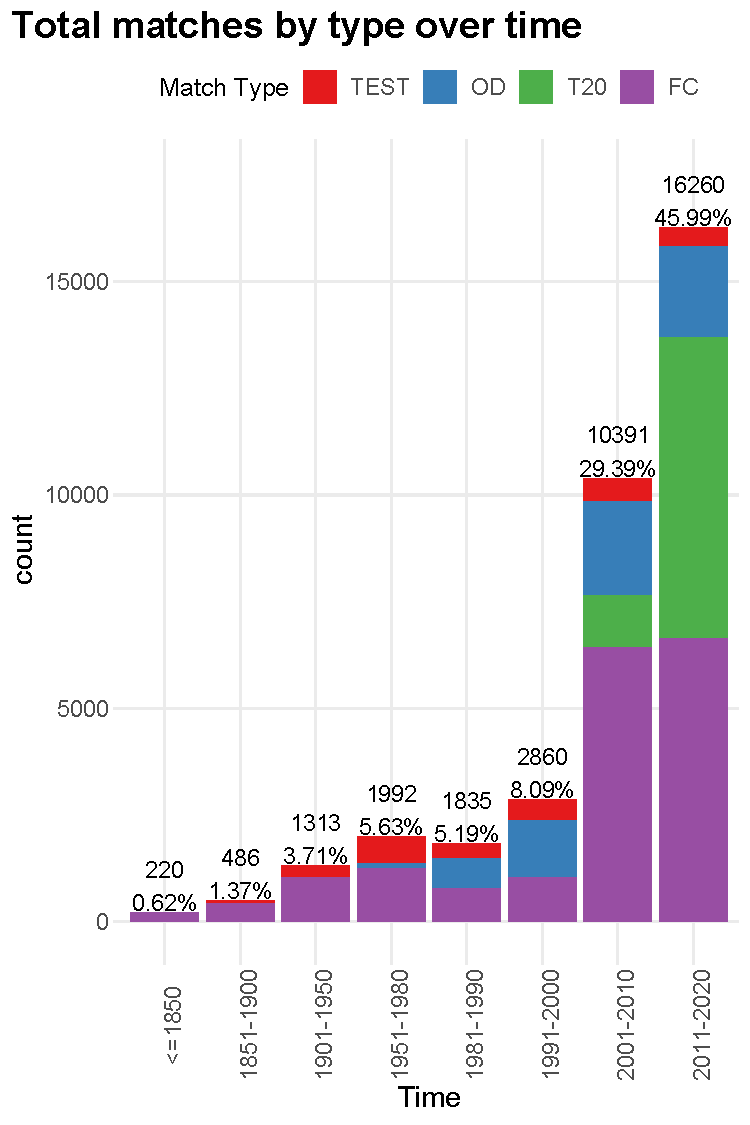
\includegraphics[width=0.6\textwidth,keepaspectratio]{output/matchcounts.pdf}
  \caption{Number of matches by format over time}
  \label{fig:timeseries_decomp}
\end{figure}


\begin{table}[b!]\centering
\begin{tabular}{llll}
 & Toss Wins & Matches & $p$ value\\ \hline
Home team & 3240 & 6377 & 0.201\\
Last toss winners & 17189 & 34283 & 0.611\\
Underdog & 2001 & 4054 & 0.423\\
Home Umpire &  2075	& 4044	& 0.098 \\
\end{tabular}
\caption{Balance \label{table: balance}}
\end{table}


% \clearpage

\begin{table}
\centering
\caption{Reduced Form Effect of Toss on win probability}

\begin{tabular}{@{\extracolsep{5pt}}lcccc} 
\\[-1.8ex]\hline \\[-1.8ex] 
\\[-1.8ex] & (1) & (2) & (3) & (4)\\ 
\hline \\[-1.8ex] 
 Win Toss & 0.018$^{***}$ & 0.017$^{***}$ & 0.017$^{***}$ & 0.017$^{***}$ \\ 
  & (0.005) & (0.005) & (0.005) & (0.004) \\ 
  Constant & 0.491$^{***}$ &  &  &  \\ 
  & (0.002) &  &  &  \\ 
 Team FE &  & $\checkmark$ & $\checkmark$ & $\checkmark$ \\ 
Match-Type FE &  &  & $\checkmark$ & $\checkmark$ \\ 
Time FE &  &  &  & $\checkmark$ \\ 
\hline &  &  &  &  \\ 
Number of Matches & 35357 & 35357 & 35357 & 35357 \\ 
\hline \\[-1.8ex] 
\end{tabular} 

\label{table:reduced_form}
\end{table}

\begin{figure}[b]
  \centering
  \figinc{output/reduced_form_by_matchtype.pdf}
  \caption{Effect of winning the toss on win probability decomposed across different
  match types, over time, and by continent.}
  \label{fig:rf_het_TE}
\end{figure}

% \clearpage

\begin{figure}[b]
  \centering
  \figinc{output/reduced_form_by_format_overtime.pdf}
  \caption{Effect of winning the toss on win probability decomposed by format over time}
  \label{fig:rf_het_TE2}
\end{figure}

\begin{figure}[b]
  \centering
  \figinc{output/reduced_form_by_rank_dl_season.pdf}
  \caption{Effect of winning the toss on win probability decomposed by competitiveness, use of DL, and Seasonality}
  \label{fig:rf_het_TE3}
\end{figure}

\begin{figure}
    \centering
    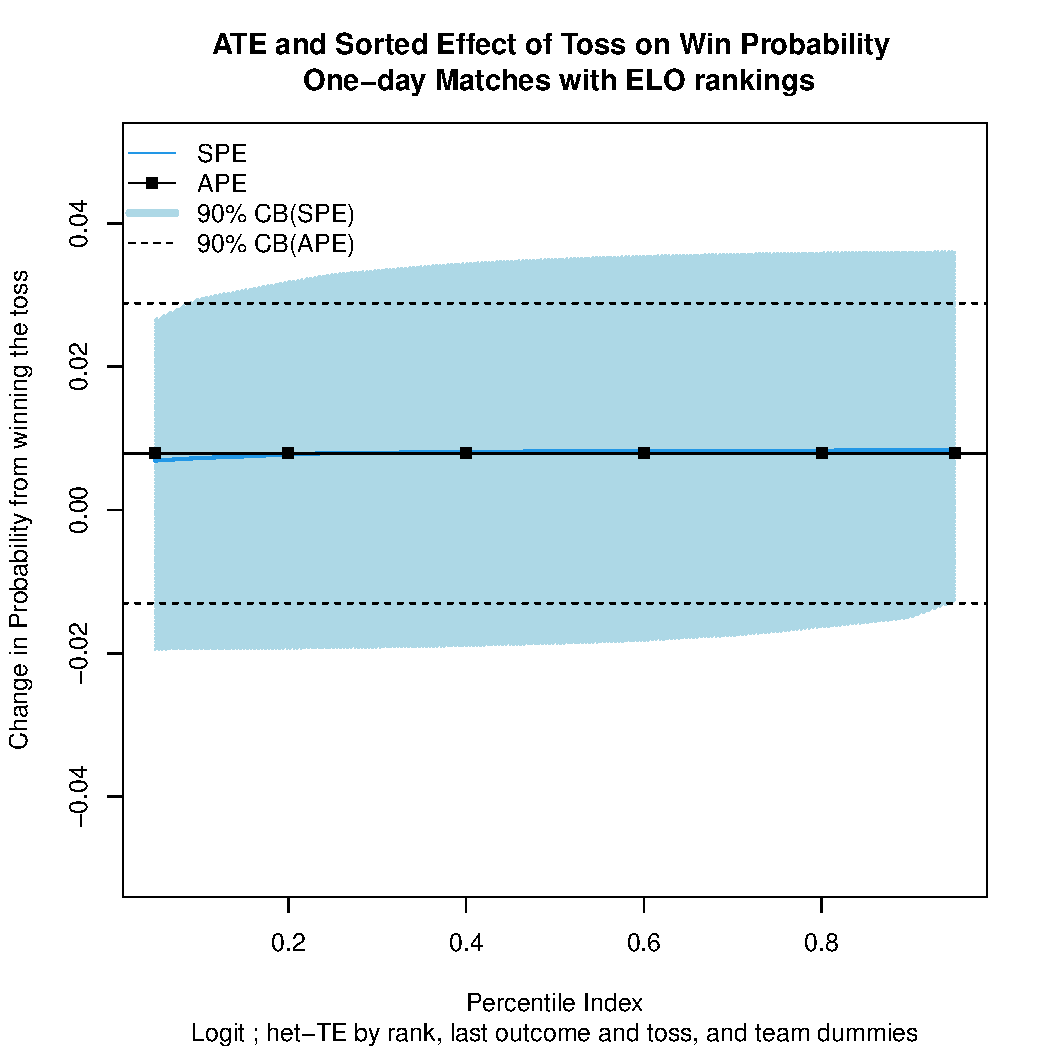
\includegraphics[width=0.5\textwidth]{output/het_rank_te_odi.pdf}
    \caption{Treatment effect heterogeneity by ranking, toss and win history, and team dummies. Minimal evidence of effect heterogeneity}
    \label{fig:omni_het_odi}
\end{figure}

\begin{figure}
    \centering
    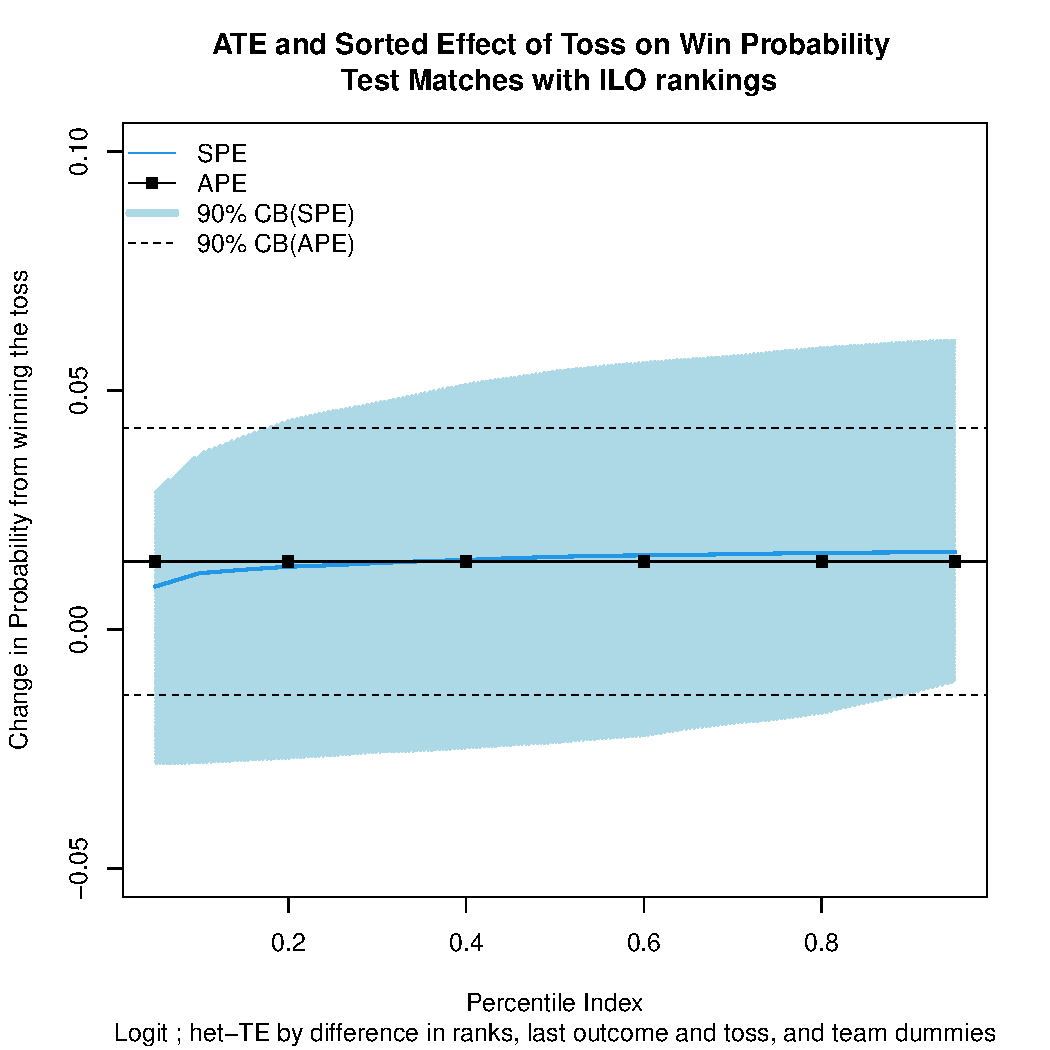
\includegraphics[width=0.5\textwidth]{output/het_rank_te_test.pdf}
    \caption{Treatment effect heterogeneity for test matches by ranking, toss and win history, and team dummies. Minimal evidence of effect heterogeneity}
    \label{fig:omni_het_test}
\end{figure}



% \clearpage

\begin{table}
\scriptsize
\centering
\caption{Batting first and win probability}

\begin{tabular}{@{\extracolsep{5pt}}lccccccc} 
\\[-1.8ex]\hline \\[-1.8ex] 
 & \multicolumn{3}{c}{OLS} & First-Stage & \multicolumn{3}{c}{IV} \\ 
\\[-1.8ex] & (1) & (2) & (3) & (4) & (5) & (6) & (7)\\ 
\hline \\[-1.8ex] 
 Bat First & $-$0.016$^{***}$ & 0.002 & $-$0.039$^{***}$ &  &  &  &  \\ 
  & (0.005) & (0.006) & (0.007) &  &  &  &  \\ 
  Win Toss &  &  &  & 0.130$^{***}$ &  &  &  \\ 
  &  &  &  & (0.005) &  &  &  \\ 
  Bat First (IV) &  &  &  &  & 0.139$^{***}$ & 0.134$^{***}$ & 0.134$^{***}$ \\ 
  &  &  &  &  & (0.036) & (0.036) & (0.036) \\ 
  Constant & 0.508$^{***}$ & 0.499$^{***}$ & 0.519$^{***}$ & 0.435$^{***}$ & 0.430$^{***}$ &  &  \\ 
  & (0.002) & (0.003) & (0.004) & (0.003) & (0.018) &  &  \\ 
 Sample & All & TW bats & TW fields & All & All & All & All \\ 
FS F-Stat &  &  &  &  &  & 604.71 & 579.95 \\ 
Team FE &  &  &  &  &  & $\checkmark$ & $\checkmark$ \\ 
Match-Type FE &  &  &  &  &  & $\checkmark$ & $\checkmark$ \\ 
Decade FE &  &  &  &  &  &  & $\checkmark$ \\ 
\hline &  &  &  &  &  &  &  \\ 
Number of Matches & 35357 & 19971 & 15386 & 35357 & 35357 & 35357 & 35357 \\ 
\hline \\[-1.8ex] 
\end{tabular} 

\label{table:iv_table}
\end{table}


\begin{figure}
 \centering
 \figinc{output/first_stage_by_matchtype.pdf}
 \caption{Toss effects on choice to bat decomposed across different match
 types, timing, and continent.}
 \label{fig:fs_het_TE1}
\end{figure}

\begin{figure}
 \centering
 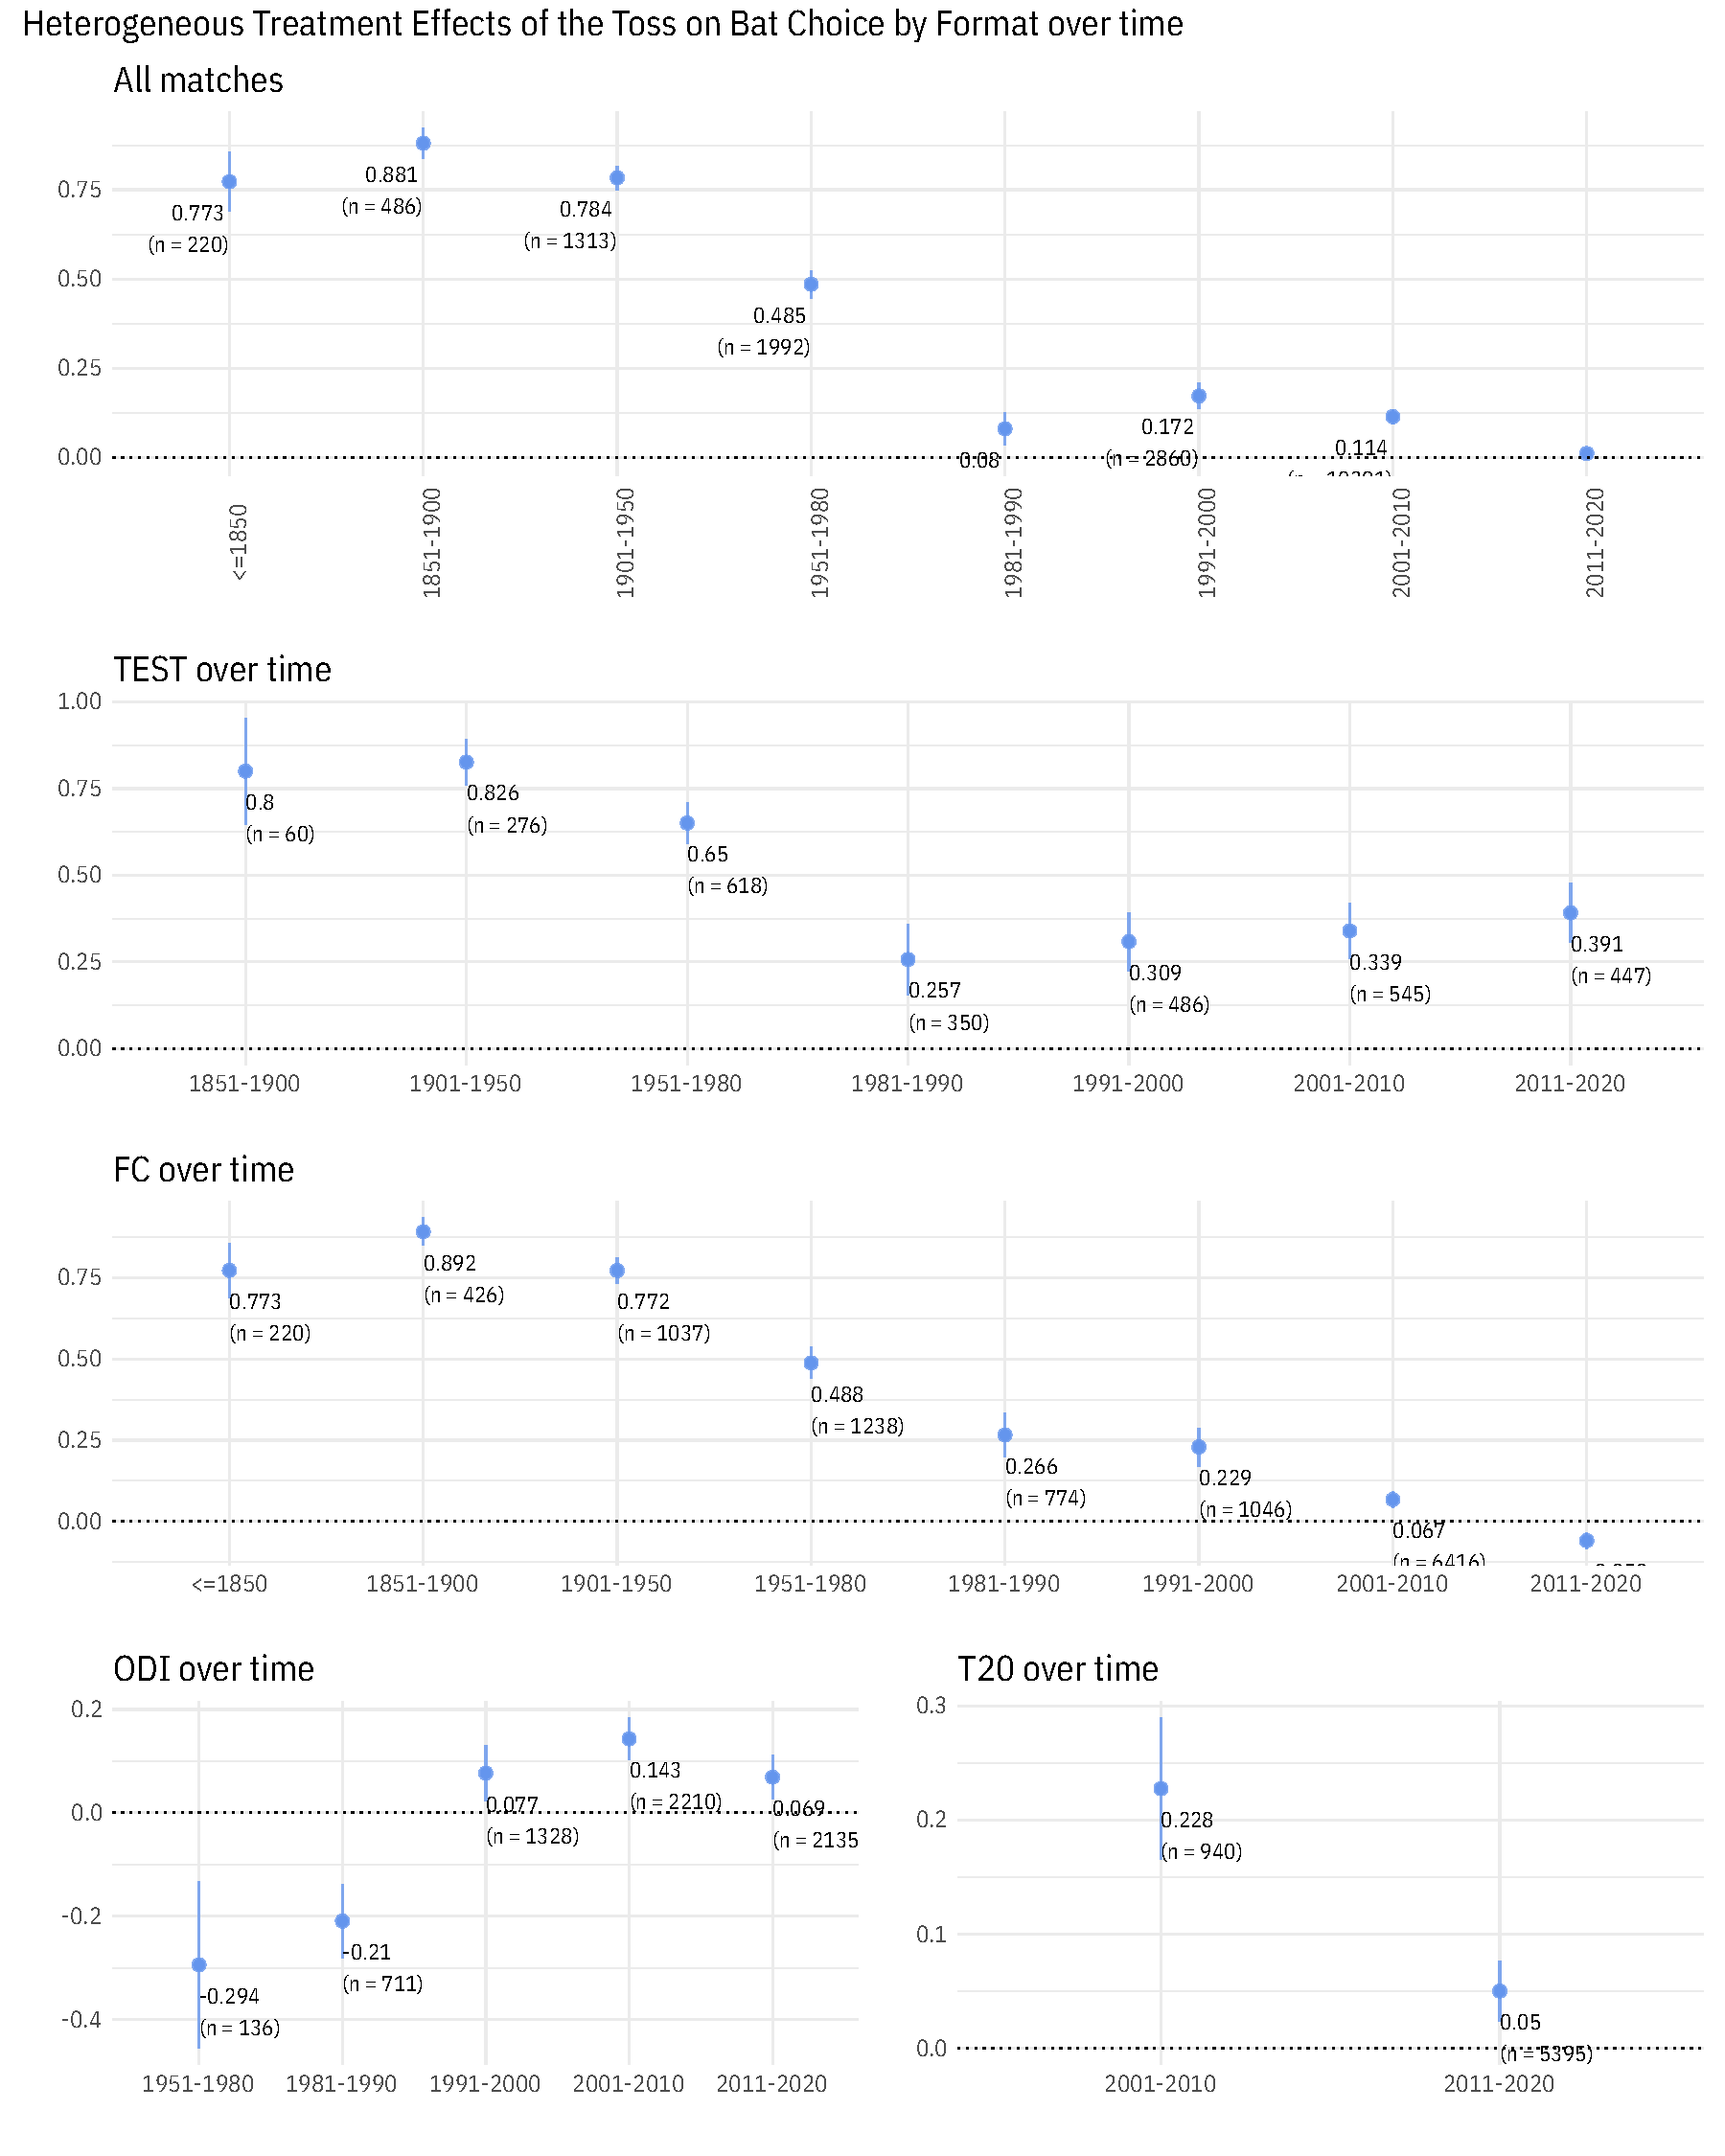
\includegraphics[width=\textwidth,keepaspectratio]{output/first_stage_by_format_overtime.pdf}
 \caption{Toss effects on choice to bat decomposed across different formats
 over time}
 \label{fig:fs_het_TE2}
\end{figure}


\begin{figure}
 \centering
 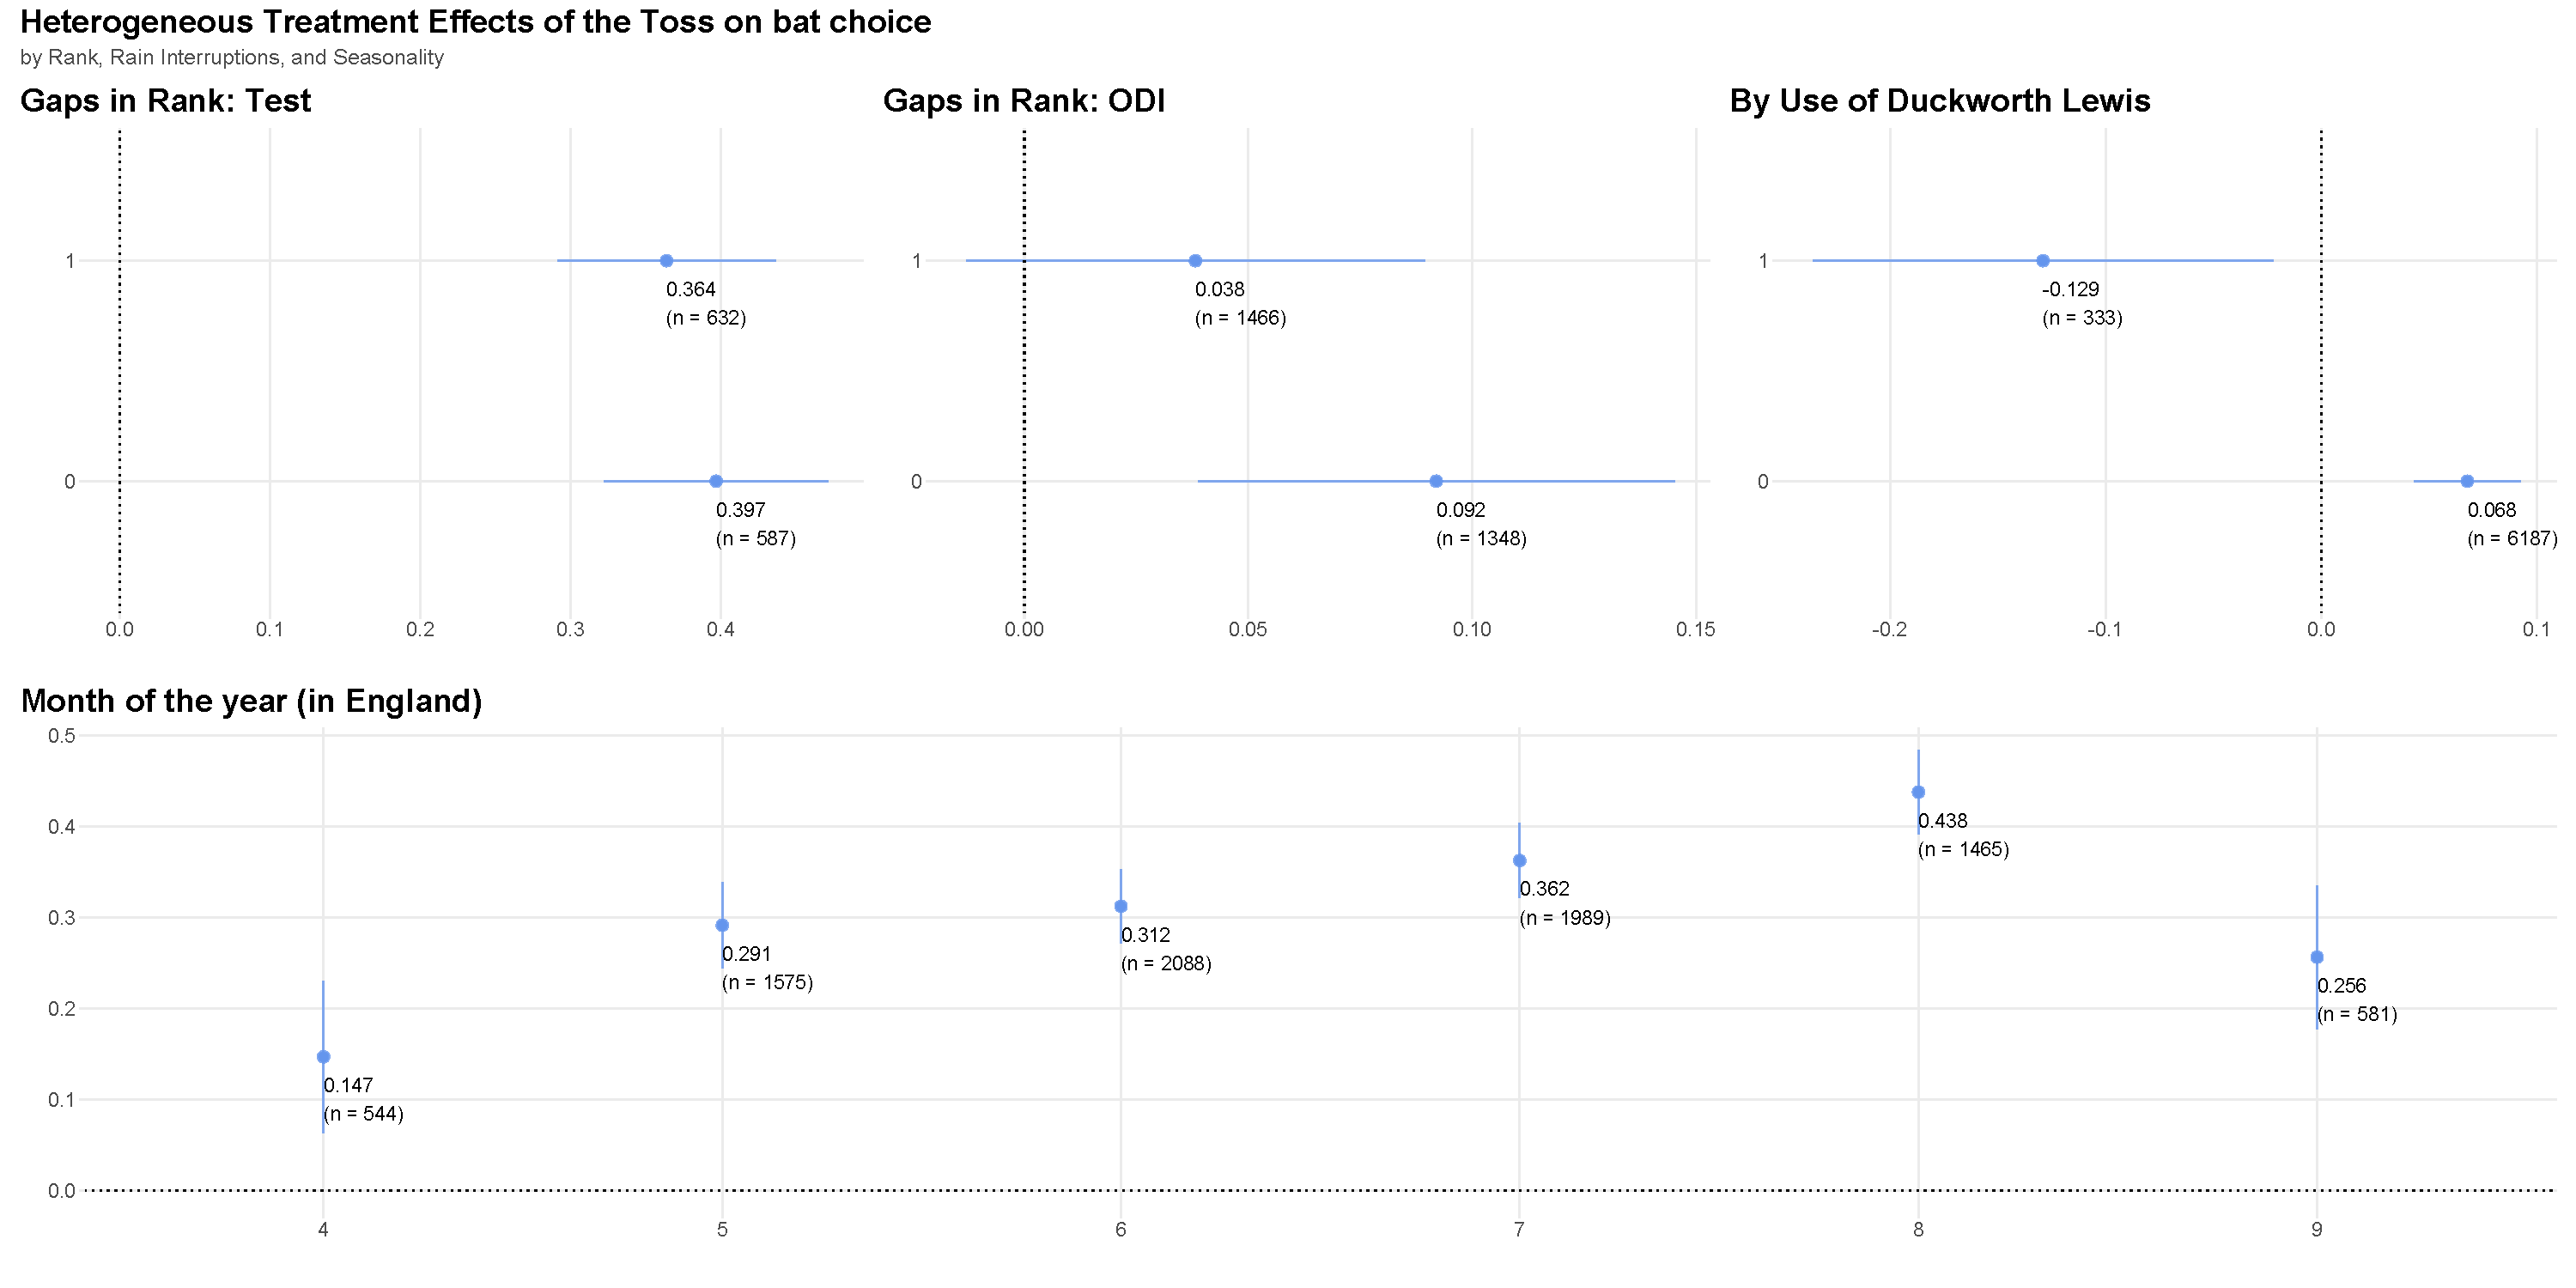
\includegraphics[width=0.9\textwidth,keepaspectratio]{output/first_stage_by_rank_dl_season.pdf}
 \caption{Toss effects on choice to bat decomposed by ranking differences, rain-interruptions, and season (in England)}
 \label{fig:fs_het_TE3}
\end{figure}

%\begin{figure}
%  \centering
%  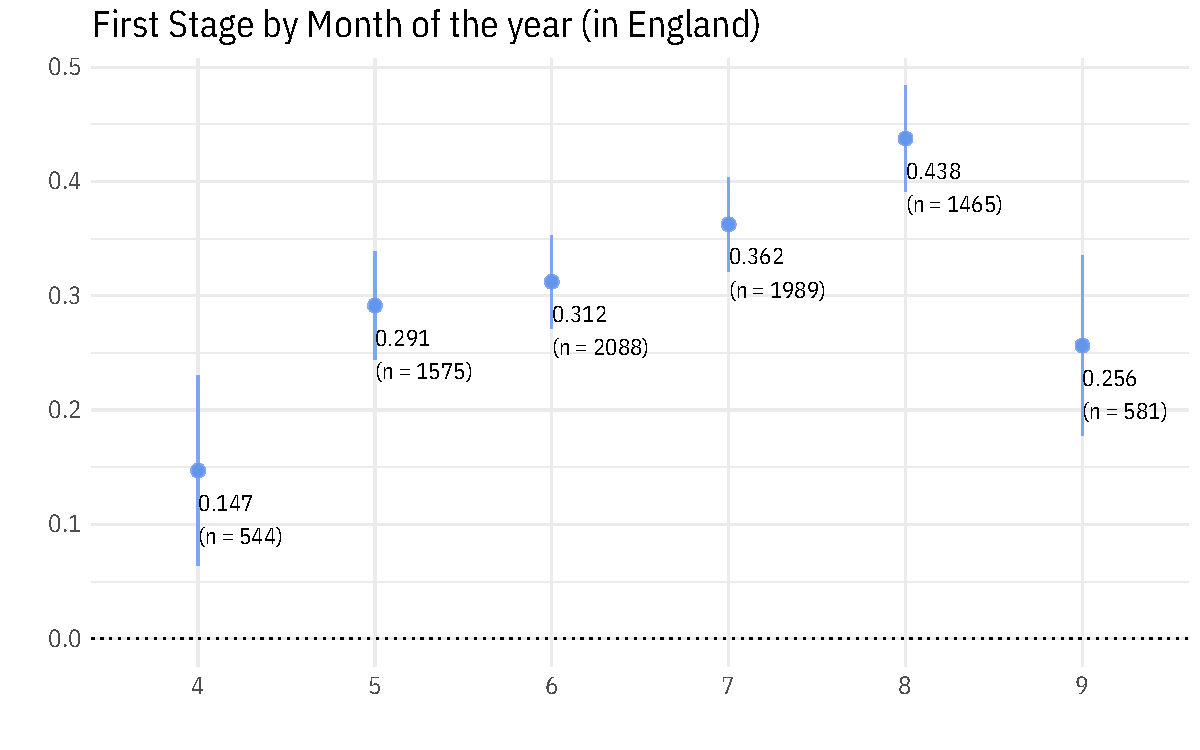
\includegraphics[width=0.9\textwidth,keepaspectratio]{output/first_stage_season.pdf}
%  \caption{First stage (probability of choosing to bat first after winning the toss) by month in England}
%  \label{fig:first_stage_seasonality}
%\end{figure}
%
%
%\clearpage
%
%
%\begin{table}[!htb]
%    \caption*{}
%    \begin{minipage}{.5\linewidth}
%      \caption{Team Characteristics}
%      \centering
%        \begin{tabular}{l|r}
%        % \label{table:kappa_res1}
%        \hline
%        & $\Ol{X}$\\
%        \hline
%        underdog & 0.52\\
%        \hline
%        day/night & 0.78\\
%        \hline
%        home & 0.42\\ \hline \hline \\
%        \textbf{continent} & \\
%        \hline
%        africa & 0.11\\
%        \hline
%        asia & 0.62\\
%        \hline
%        europe & 0.03\\
%        \hline
%        oceania & 0.24\\
%        \hline
%        \end{tabular}
%    \end{minipage}%
%    \begin{minipage}{.5\linewidth}
%      \centering
%        \caption{Team}
%        \begin{tabular}{l|r}
%        % \label{table:kappa_res2}
%        \hline
%        team & $\Ol{X}$\\
%        \hline
%        australia & 0.27\\
%        \hline
%        bangladesh & 0.01\\
%        \hline
%        england & 0.15\\
%        \hline
%        india & 0.15\\
%        \hline
%        kenya & 0.02\\
%        \hline
%        new zealand & 0.00\\
%        \hline
%        pakistan & 0.15\\
%        \hline
%        south africa & 0.14\\
%        \hline
%        sri lanka & 0.03\\
%        \hline
%        west indies & 0.04\\
%        \hline
%        zimbabwe & 0.04\\
%        \hline
%        \end{tabular}
%    \end{minipage}
%\end{table}
%
%

%\renewcommand{\mkbibnamefamily}[1]{\textsc{#1}}
%\printbibliography
%
%\appendix



\end{document}
